\chapter{Hierarchical Control for Head-to-Head Racing} \label{chapter:hier}
\section{Hierarchical Control Design}
% \begin{figure}
%   \centering
%   \includegraphics[height=0.5\textheight]{Figures/ControlStructureVertical.png}
%   \caption{The continuous dynamic game (top) transformed into the high-level discrete game (middle). The discrete game solution created by the high-level planner (highlighted in green) is tracked by the low-level planner (bottom).}
%   \label{fig:overall_control}
% \end{figure}
\begin{figure*}
  \centering
%   \includegraphics[width=\textwidth]{Figures/FormulationBreakdown.png}
    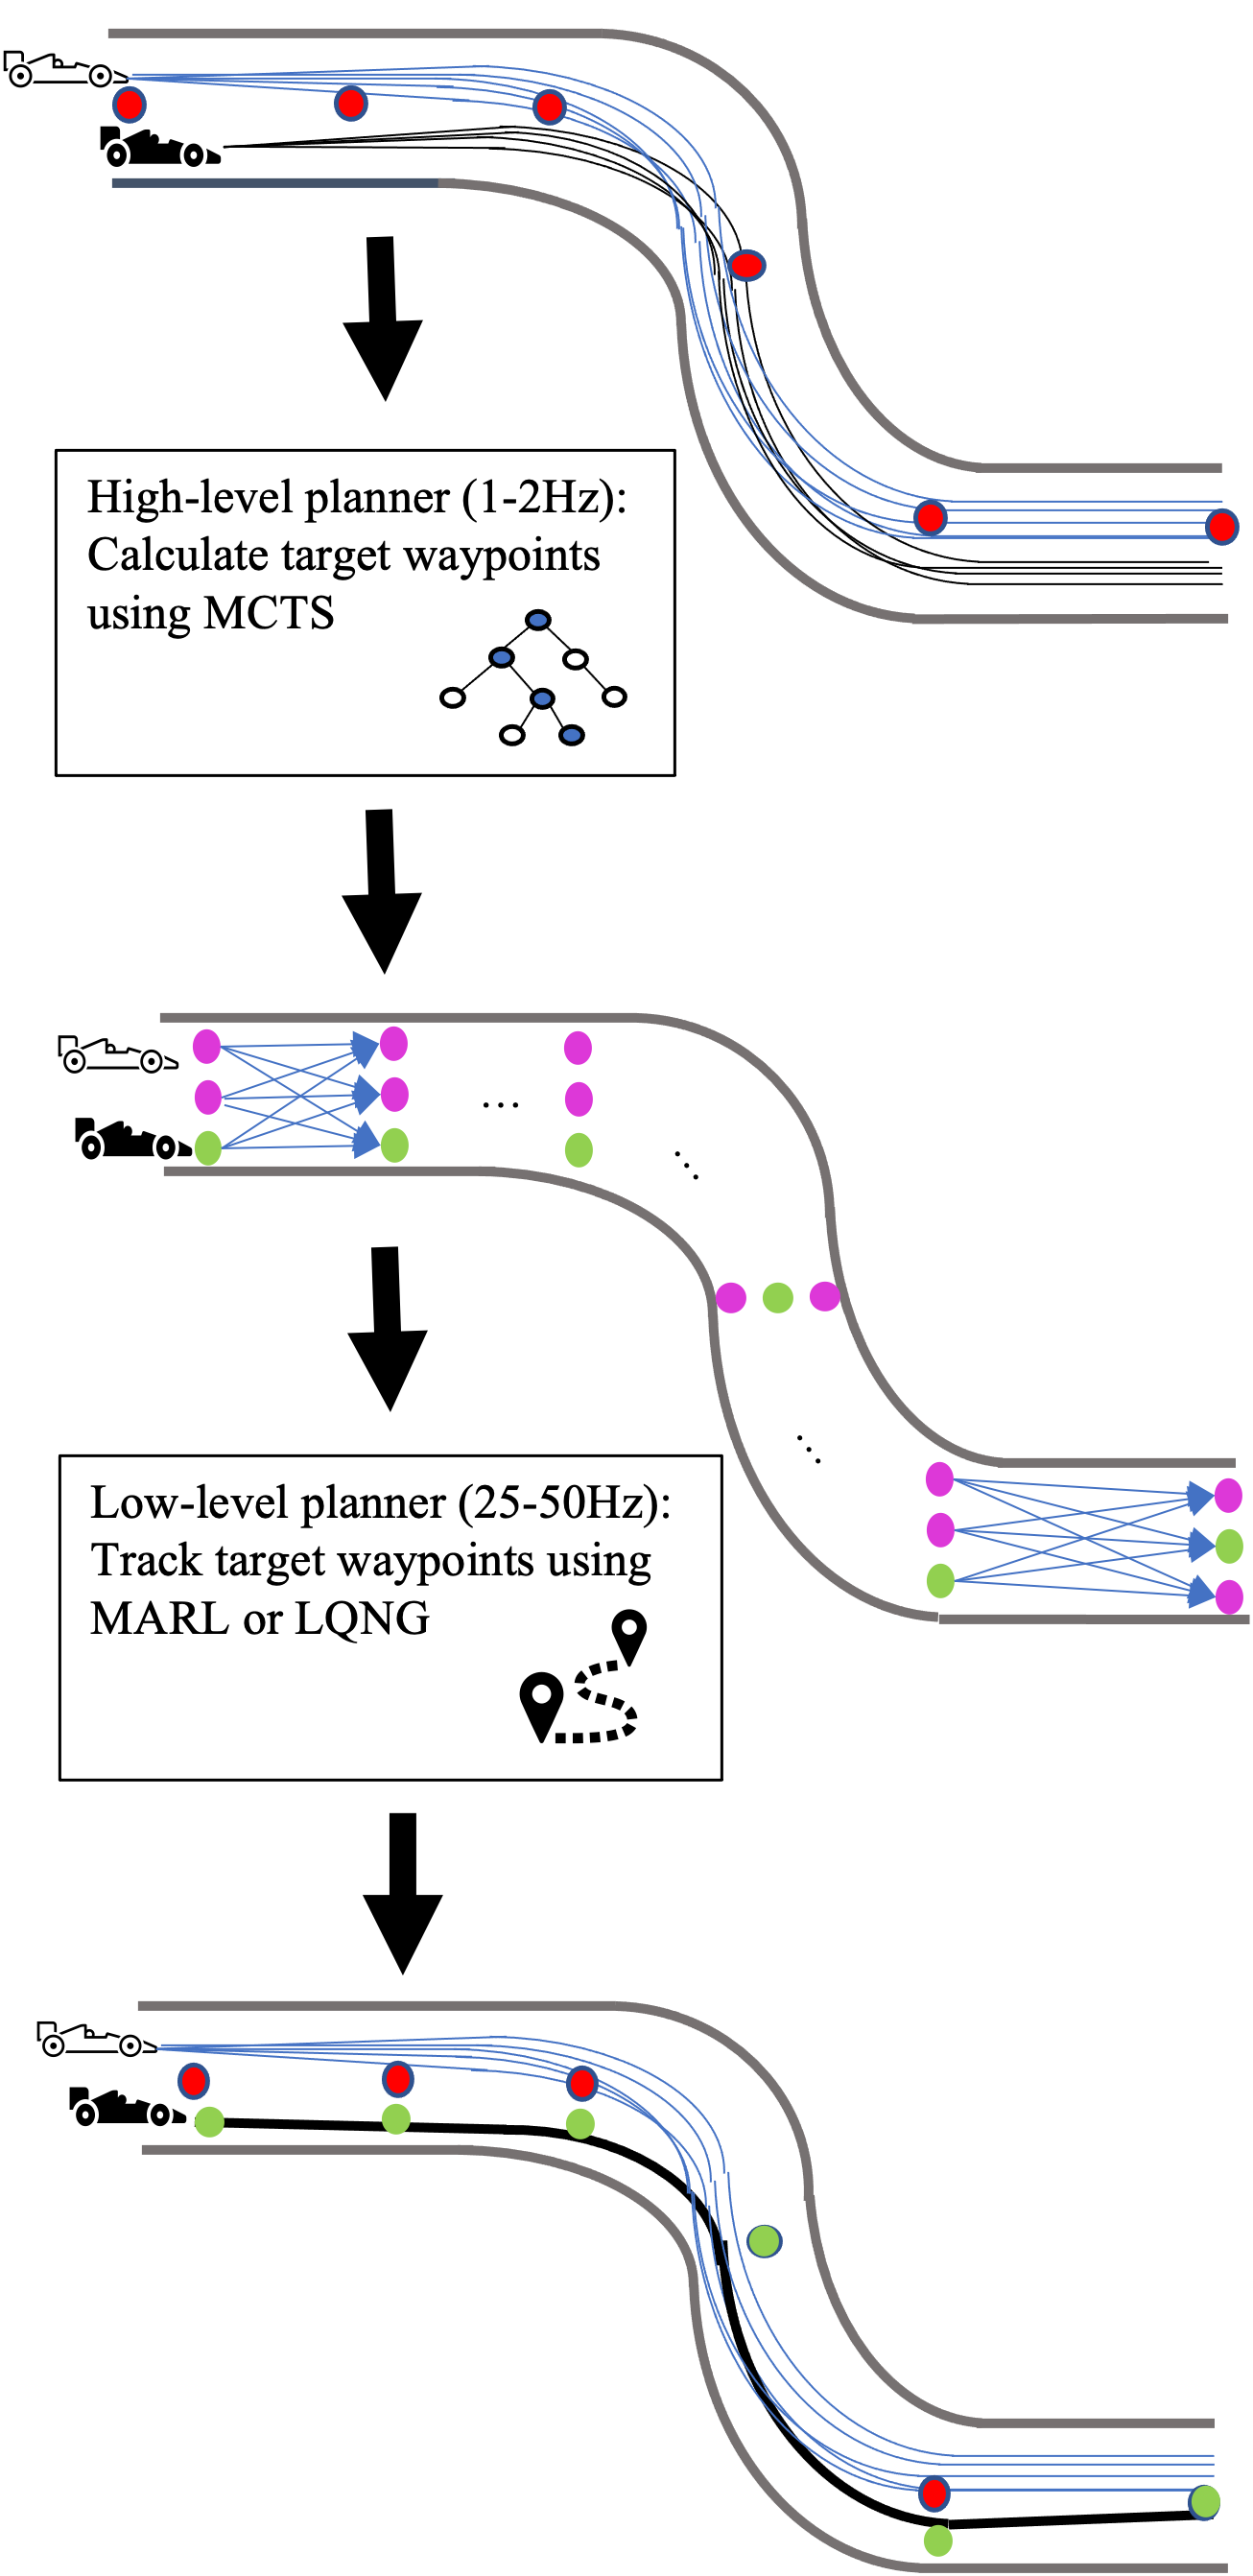
\includegraphics[height=0.8\textheight]{Figures/FormulationBreakdownVert.png}
  \caption{The uncountably infinite trajectories of the general game (top) discretized by the high-level planner (middle). The sequence of target waypoints calculated by the high-level planner (in green) is tracked by the low-level planner (bottom) and converges to a continuous trajectory (in black).}
  \label{fig:overall_control}
\end{figure*}
Traditional optimization-based control methods cannot easily be utilized for the general multi-agent racing game formulated with realistic safety and fairness rules. The rules involve nonlinear constraints over both continuous and discrete variables, and a mixed-integer non-linear programming algorithm would be unlikely to run at rates of \SI{25}{\hertz}-\SI{50}{\hertz} for precise control. This inherent challenge encourages utilizing a method such as deep reinforcement learning or trying to solve the game using short horizons. 

However, we propose a hierarchical control design involving two parts that work to ensure all of the rules are followed while approximating long-term optimal choices. The high-level planner transforms the general formulation into a game with discrete states and actions where all of the discrete rules are naturally encoded. The solution provided by the high-level planner is a series of discrete states (i.e waypoints) for each player, which satisfies all of the rules. Then, the low-level planner solves a simplified version of the racing game with an objective putting greater emphasis on tracking a series of waypoints and smaller emphasis on the original game-theoretic objective and a simplified version of the rules. Therefore, this simplified formulation can be solved by an optimization method in real-time or be trained in a neural network when using a learning-based method. 
%This control design assumes that if the series of waypoints produced by the high-level planner is guaranteed to follow the rules, then the control inputs generated by the waypoint tracking low-level planner will also satisfy the rules of the original game when applied to the actual underlying system. 
% Figure \ref{fig:overall_control} visualizes the overall control architecture.
\subsection{High-Level Planner}
% Describe High-Level Game (states, transitions, rewards)
The high-level planner constructs a turn-based discrete, dynamic game that is an approximation of the general game \eqref{eq:gen_obj}-\eqref{eq:gen_lane_lim}. Continuous components of a players' states are broken into discrete ``buckets'' (e.g., speed between \SI{2}{\meter\per\second} and \SI{4}{\meter\per\second}, tire wear between 10\% and 15\%). In addition, $\lambda$ (which is the number of lanes) points around each checkpoint are chosen along a line perpendicular to the direction of travel where each point evaluates to a unique lane ID on the track when passed into function $z(\cdot)$ defined in the general formulation. The left and center of Figure \ref{fig:overall_control} visualize the checkpoints in the original, continuous formulation (in red) expanded into three discrete lanes (green or purple) for the high-level game.  

The players' actions are defined by pairs of lane ID, resolving to a target location near the next checkpoint, and target speed for that location. Therefore, we can apply a simplified inverse approximation of the dynamics to determine the time it would take to transition from one checkpoint to the next and estimate the remaining state variables or dismiss the action if it is dynamically infeasible. This action space also allows us to easily evaluate or prevent actions where rules of the game would be broken. By limiting choices to fixed locations across checkpoints, we ensure that the players always remain on track \eqref{eq:gen_idx_dist}. Moreover, the players' actions can be dismissed if they would violate the limit on the number of lane changes by simply checking whether choosing a lane would exceed their limits or checking if the location is a curve or straight \eqref{eq:gen_lane_lim}. Finally, other actions that could cause collisions can also be dismissed by estimating that if two players reach the same lane at a checkpoint and have a small difference in their time states, there would be a high risk of collision \eqref{eq:gen_coll_avoid}.

The game is played with each player starting at the initial checkpoint, and it progresses by resolving all players' choices one checkpoint at a time. The order in which the players take their actions is determined by the player who has the smallest time state at each checkpoint. A lower time state value implies that a player was at the given checkpoint before other players with a larger time state, so it would have made its choice at that location before the others. This ordering also implies that players who arrive at a checkpoint after preceding players observe the actions of those preceding players. Therefore, these observations can contribute to their strategic choices. Most importantly, because the ordering forces the following players to choose last, we also capture the rule that the following players (i.e. those that are ``behind'' others) are responsible for collision avoidance after observing the leading players' actions. 

% Describe objective and MCTS approach used to solve it -> waypoints
The objective of the discrete game is to minimize the difference between one's own time state at the final checkpoint and that of all other players just like the original formulation \eqref{eq:gen_obj}. Although the discrete game is much simpler than the original formulation, the state space grows as the number of actions and checkpoints increases. Therefore, we solve the game in a receding horizon manner, but our choice of the horizon (i.e. number of checkpoints to consider) extends much further into the future than an MPC-based continuous state/action space controller can handle in real time \cite{wang2019game}. In order to produce a solution to the discrete game in real-time, we use the Monte Carlo tree search (MCTS) algorithm \cite{mcts}. The solution from applying MCTS is a series of waypoints in the form of target lane IDs (which can be mapped back to positions on track) and the target velocities at each of the checkpoints for the ego player and estimates of the best response lanes and velocities by the adversarial players. 

\subsection{Low-Level Planner}
% Describe Simplified waypoint Following Game
The low-level planner is responsible for producing the control inputs, so it must operate in real-time. Because we have a long-term plan from the high-level planner, we can formulate a reduced version of the original game for our low-level planner. The low-level game is played over a shorter horizon compared to the original game of just $\delta$ steps in $\hat{\mathcal{T}} = \{1, ..., \delta\}$. We assume that the low-level planner for player $i$ has received $k$ waypoints, $\psi^i_{r^i_{1}}, ..., \, \psi^i_{r^i_{1} + k}$, from the high-level planner, and player $i$'s last passed checkpoint $r^i_*$. 
% Table \ref{tab:ll_symbols} includes the additional parameters referenced in the simplified formulation.

The low-level objective involves two components. The first is to maximize the difference between its own checkpoint index and the opponents' checkpoint indices at the end of $\delta$ steps. The second is to minimize the tracking error, $\eta^i_y$, of every passed waypoint $\psi^i_{r^i_{1}+y}$. The former component influences the player to pass as many checkpoints as possible, which suggests reaching $c_\tau$ as quickly as possible. The latter influences the player to be close to the high-level waypoints when passing each of the checkpoints. The objective also includes some multiplier $\alpha$ that balances the emphasis of the two parts. The objective is written as follows:
% Low-Level Formulation

\begin{equation} \label{eq:ll_obj}
    \min_{u^i_{1}, ..., u^i_{\delta}} (\sum^N_{j \neq i}r^j_{\delta} - (|N|-1) r^i_{\delta}) + \alpha \sum_{c={r^i_{1}}}^{{r^i_{1}}+k} \eta^i_c
\end{equation}

The players' continuous state dynamics, calculations for each checkpoint, and constraints on staying within track bounds \eqref{eq:ll_dyn}-\eqref{eq:ll_pos_dist} are effectively the same as the original formulation. 

\begin{equation} \label{eq:ll_dyn}
    x^j_{t+1} = f(x^j_{t}, u^j_t), \quad \forall \;\; t \in \hat{\mathcal{T}}, j \in N
\end{equation}
\begin{equation} \label{eq::ll_pos}
    r^j_{t+1} = p(x^j_{t+1}, r^j_t), \quad \forall \;\; t \in \hat{\mathcal{T}}, j \in N
\end{equation}
\begin{equation} \label{eq::ll_pos_init}
    r^j_{1} = r^j_*, \quad \forall\;\; j \in N
\end{equation}
\begin{equation} \label{eq:ll_pos_dist}
    q(x^m_{t}) \leq w, \quad \forall \;\; t \in \hat{\mathcal{T}}, j \in N
\end{equation}

The collision avoidance rules are simplified to just maintaining a minimum distance $s_0$ as the high-level planner would have already considered the nuances of rear-end collision avoidance responsibilities in \eqref{eq:gen_coll_avoid}. As a result, we require the following constraint to hold for all $t \in \mathcal{T}$, $j \in N$, and $k \in N \setminus \{j\}$:
\begin{equation} \label{eq:ll_coll_avoid}
    d(x^j_{t}, x^k_t) \geq s_0
\end{equation}

Finally, we define the dynamics of the waypoint error, $\eta^i_y$, introduced in the objective. It is equivalent to the accumulated tracking error of each target waypoint that player $i$ has passed using a function $h: X\times X \rightarrow \mathbb{R}$ that measures the distance. If a player has not passed a waypoint, then the variable indexed by that waypoint is set to 0. The variable's dynamics are expressed by the following constraint:

\begin{multline} \label{eq:ll_wp_err}
    \eta^i_y = \begin{cases} \sum_{t}^{\Hat{\mathcal{T}}} h(x^i_t, \psi^i_{c})  & \text{if } \exists \; r^i_t \geq y \\
    0 & \text{otherwise}
    \end{cases} \\ \forall \; y \in \{r^i_{1}, ..., r^i_{1} + k\}
\end{multline}

% Low-Level params table
% \begin{table}[b]
% \centering
% \caption{Additional symbols in low-level formulation}
% \begin{tabular}{p{0.15\linewidth}|p{0.75\linewidth}}  \label{tab:ll_symbols}
% Symbol & Value  \\ 
% \hline
% $\hat{\mathcal{T}}$ & Set of steps in the game \\
% $\hat{\delta}$ & Shortened horizon \\
% $\alpha$      &   Weight parameter in objective emphasizing importance of hitting trajectory waypoints    \\
% $\psi^i_c$      &   Waypoint for player $i$ to target when passing checkpoint index $c$ \\
% $\eta^i_c$  &  Distance of player $i$'s closest approach to the waypoint $\psi^i_c$ \\ 
% $h(x^i_{t}, \psi^i_c)$  &  Function distance of player $i$'s state to waypoint $\psi^i_c$ \\  
% \end{tabular}
% \end{table}
% Describe Low-Level Formulation
This simplified formulation is similar to the general formulation. However, the constraints introduced by the complex fairness and safety rules are dropped since they are considered by the high-level planner. The center and right of Figure \ref{fig:overall_control} show how the waypoints from the high-level planner (in green) are approximately tracked by the low-level planner producing a continuous trajectory (in black). We consider two methods to solve this low-level formulation. The first method develops a reward structure to represent this simplified formulation for a multi-agent reinforcement learning (MARL) controller. The second method further simplifies the low-level formulation into a linear-quadratic Nash game (LQNG) to compute the control inputs. 

\subsubsection{Multi-Agent Reinforcement Learning Controller}
% RL objective/reward structure for this game
Designing the MARL controller primarily involves shaping a reward structure that models the low-level formulation. The RL agent is rewarded for the following behaviors that would improve the objective function \eqref{eq:ll_obj}:
\begin{itemize}
    \item Passing a checkpoint with an additional reward for being closer to the target lane and velocity.
    \item Minimizing the time between passing two checkpoints.
    \item Passing as many checkpoints in the limited time.
\end{itemize}
On the other hand, the agent is penalized for actions that would violate the constraints:
\begin{itemize}
    \item Swerving too frequently on straights \eqref{eq:gen_lane_lim}.
    \item Going off track or hitting a wall \eqref{eq:ll_pos_dist}.
    \item Colliding with other players \eqref{eq:ll_coll_avoid} with additional penalty if the agent is responsible for avoidance \eqref{eq:gen_coll_avoid}. 
\end{itemize}

The rewards capture our low-level formulation objective \eqref{eq:ll_obj} to pass as many checkpoints as possible while closely hitting the lane and velocity targets \eqref{eq:ll_wp_err}. The penalties capture the on-track \eqref{eq:ll_pos_dist} and collision avoidance \eqref{eq:ll_coll_avoid} constraints. However, the penalties also reintroduce the original safety and fairness from the original general game that were simplified away from the low-level formulation \eqref{eq:gen_coll_avoid} and \eqref{eq:gen_lane_lim}. Because these rules are inherently met by satisfying the objective of reaching the high-level planner's waypoints, their penalties have the weights set much lower than other components of the reward structure. However, we still incorporate the original form of these penalties to reinforce against the possibility that the ego player might be forced to deviate far away from the high-level plan.

The agents' observations include perfect state information of all players and local observations consisting of 9 LIDAR rays spaced over a 180\textdegree{} field of view centered in the direction that the player is facing.

\subsubsection{Linear-Quadratic Nash Game Controller}
% Linear approximation of the waypoint following game
Our second low-level approach solves an LQNG using the Coupled Riccati equations \cite{basar}. This method involves further simplifying the low-level formulation into a structure with a quadratic objective and linear dynamics. The continuous state is simplified to just four variables: $x$ position, $y$ position, $v$ velocity, and $\theta$ heading. The control inputs $u^i_t$ are also explicitly broken into acceleration, $a^i_t$, and yaw-rate, $e^i_t$. The planning horizon is reduced to $\Bar{\delta}$ where $\Bar{\delta} << \delta < T$. To construct our quadratic objective for player $i$, we break it into three components. The first is to minimize the distance to the upcoming target waypoint from the high-level planner $\Bar{\psi}^i$ calculated by the following equation:
\begin{multline} \label{eq:lqng_obj1}
\upsilon^i(\rho_1, \rho_2,\rho_3) =  \sum_{t = 1}^{\Bar{\delta}} (\rho_1((x^i_{t} - \Bar{\psi}^i_x)^2 + (y^i_{t} - \Bar{\psi}^i_y)^2) \\   \quad + \rho_2 (v^i_{t} - \Bar{\psi}^i_v)^2 
 + \rho_3 (\theta^i_{t} - \Bar{\psi}^i_\theta)^2)
\end{multline}

The second component is to maximize each opponent's distance from the location of estimated target waypoints $\Bar{\psi^j}$ calculated by the following equation:
\begin{equation} \label{eq:lqng_obj2}
    \phi^i(\Bar{\psi}^j, \rho) = \sum_{t = 1}^{\Bar{\delta}} \rho((x^j_{t} - \Bar{\psi}^j_x)^2 + (y^j_{t} - \Bar{\psi}^j_y)^2)
\end{equation}

We drop all of the constraints with the exception of collision avoidance, and it is incorporated as the third component and penalty term in the objective where the distance to each opponent should be maximized. This term is calculated by the following equation:
\begin{equation} \label{eq:lqng_obj3}
    \chi^i(x^j_t, y^j_t, \rho) = \sum_{t = 1}^{\Bar{\delta}} \rho((x^j_{t} - x^i_{t})^2 + (y^j_{t} - y^i_{t})^2)
\end{equation}

The final quadratic objective aggregates \eqref{eq:lqng_obj1}-\eqref{eq:lqng_obj3} using weight multipliers ($\rho_i$) to place varying emphasis on the components as follows:

\begin{small}
\begin{multline} \label{eq:lqng_obj}
    \min_{a^i_{1}, e^i_{1}, ..., a^i_{\Bar{\delta}}, e^i_{\Bar{\delta}}}
    \upsilon^i(\rho_1, \rho_2,\rho_3)
    -\sum_{j \neq i}^{N}  (\phi^i(\Bar{\psi}^j, \rho_4) - \chi^i(x^j_t, y^j_t, \rho_5))
\end{multline}
\end{small}

Finally, the linear dynamics are time invariant and apply for all players $j \in N$:

\begin{small}
\begin{multline} \label{eq:lqng_dyn}
\begin{bmatrix}
x^j_{t+1} \\
y^j_{t+1} \\
v^j_{t+1} \\
\theta^j_{t+1} \\
\end{bmatrix} = 
\begin{bmatrix} 
	1 & 0 & -\sin(\theta^j_{t_0})\Delta t & \cos(\theta^j_{t_0})\Delta t\\
	0 & 1 & \cos(\theta^j_{t_0})\Delta t & \sin(\theta^j_{t_0})\Delta t\\
	0 & 0 & 1 & 0\\
	0 & 0 & 0 & 1\\
	\end{bmatrix}
\begin{bmatrix}
x^j_{t} \\
y^j_{t} \\
v^j_{t} \\
\theta^m_{t} \\
\end{bmatrix} \\ +
\begin{bmatrix} 
	0 & 0 \\
	0 & 0 \\
	\Delta t & 0 \\
	0 & \Delta t \\
	\end{bmatrix}
	\begin{bmatrix} 
	a^j_t  \\
	e^j_t \\
	\end{bmatrix}
\end{multline}
\end{small}
\section{Experimental Setup}
The high-level planner is paired with each of the two low-level planners discussed. We refer to our two hierarchical design variants as MCTS-RL and MCTS-LQNG. 
\subsection{Baseline Agents}
To measure the importance of our design innovations, we also consider three baseline controllers to resemble the other methods developed in prior works.  
\subsubsection{End-to-End Multi-Agent Reinforcement Learning}
The end-to-end MARL controller, referred to as ``E2E," represents the pure learning-based methods such as that of \cite{sonyai}. This controller has a similar reward/penalty structure as our low-level controller, but its observation structure is slightly different. Instead of observing the sequence of upcoming states as calculated by a high-level planner, E2E only receives the subsequence of locations from $\{c_i\}_{i=1}^{\tau}$ that denote the center of the track near the agent. As a result, it is fully up to its neural networks to learn how to plan strategic and safe moves. 

\subsubsection{Fixed Trajectory Linear-Quadratic Nash Game}
The fixed trajectory LQNG controller, referred to as ``Fixed-LQNG," uses the same LQNG low-level planner as our hierarchical variant, but it instead tracks a fixed trajectory around the track. This fixed trajectory is a racing line that is computed offline for a specific track using its geometry and parameters of the vehicle as seen in prior works \cite{vazquez2020optimizationbased, graphtraj}. However, the online tracking involves game-theoretic reasoning rather than single-agent optimal control in the prior works.

\subsubsection{Fixed Trajectory Multi-Agent Reinforcement Learning}
The fixed trajectory MARL controller, referred to as ``Fixed-RL," is a learning-based counterpart to Fixed-LQNG. Control inputs are computed using a deep RL policy trained to track precomputed checkpoints that are fixed prior to the race.  
\subsection{Controller Implementations}
% Implemented in Unity, used ML-Agents library for RL training
Our controllers are implemented\footnote{\codeurl} in the Unity Game Engine. Screenshots of the simulation environment are shown in Figure \ref{fig:experiment_tracks}. We extend the Karting Microgame template \cite{microkarting} provided by Unity. The kart physics from the template is adapted to include cornering limitations and tire wear percentage. Tire wear is modeled as an exponential decay curve that is a function of the accumulated angular velocity endured by the kart. This model captures the concept of losing grip as the tire is subjected to increased lateral loads. Multi-agent support is also added to the provided template in order to race the various autonomous controllers against each other or human players. The high-level planners run at \SI{1}{\hertz}, and low-level planners run at \SI{50}{\hertz}. Specifically, $\Bar{\delta}$ is set to \SI{0.06}{\second} for the LQNG planner. The implementation of the learning-based agents utilizes a library called Unity ML-Agents \cite{mlagents}. All of the learning-based control agents are trained using proximal policy optimization and self-play implementations from the library. They are also only trained on two sizes of oval-shaped tracks with the same number of training steps. 

% Two Tracks, 50 races head to head each
Our experiments include head-to-head racing on a basic oval track (which the learning-based agents were trained on) and a more complex track shown in Figure \ref{fig:experiment_tracks}. Specifically, the complex track involves challenging track geometry with turns whose radii change along the curve, tight U-turns, and turns in both directions. To be successful, the optimal racing strategy requires some understanding of the shape of the track along a sequence of multiple turns. Every pair of controllers competes head-to-head in 50 races on both tracks. The dynamical parameters of each player's vehicle are identical, and the players start every race at the same initial checkpoint. The only difference in their initial states is the lane in which they start. In order to maintain fairness with respect to starting closer to the optimal racing line, we alternate the starting lanes between each race for the players.
\begin{figure}
  \centering
  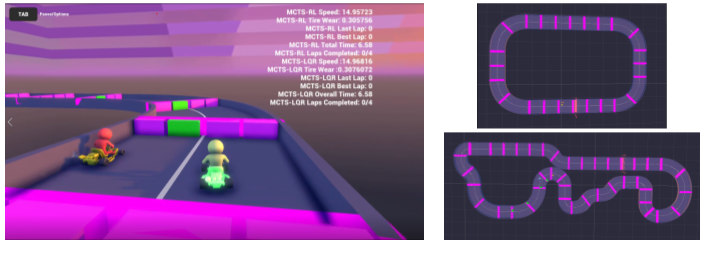
\includegraphics[width=0.4\textwidth]{Figures/UnityEnvironment.png}
  \caption{Kart racing environment from a racer's perspective (left), a bird's eye view of the oval track (right-top), and the complex track (right-bottom) in the Unity environment. The purple boxes visualize the lanes across checkpoints along the track, and the highlighted green boxes show planned waypoints determined by the hierarchical controllers.}
  \label{fig:experiment_tracks}
\end{figure}
\section{Head-to-Head Racing Results}
